\input ../preamble

\begin{document}

{\Huge

  \centerline{\bf TTIC 31230, Fundamentals of Deep Learning}
  \bigskip
  \centerline{David McAllester, Winter 2018}
  \vfill
  \centerline{\bf Deep Graphical Models I}
  \vfill
  \vfill
  \centerline{Exponential Softmax}
  \vfill
  \centerline{Sufficient Statistics}
  \vfill
  \centerline{Belief Propagation}
  
\vfill


\slide{Consider Colorization}

\centerline{\includegraphics[height = 2in]{../images/colorization}}

$x$ is a black and white image.

\vfill
$y$ is a color image drawn from $\pop(y|x)$.

\vfill
$\hat{y}$ is an arbitrary color image.

\vfill
$Q_\Phi(\hat{y}|x)$ is the probability that model $\Phi$ assigns to the color image $y$ given black and white image $x$.

\slide{Cross Entropy Training}

\centerline{\includegraphics[height = 2in]{../images/colorization}}

\vfill
\begin{eqnarray*}
\Phi^* & =  & \argmin_\Phi \;\;E_{(x,y) \sim \pop}  -\log Q_\Phi(y|x)
 \end{eqnarray*}

\slide{Auto-Regressive Models are Tractable}

\centerline{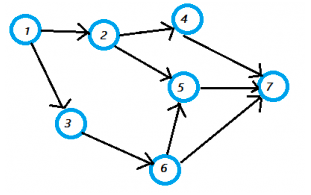
\includegraphics[height=1.5in]{../images/DAG} \hspace{1in} 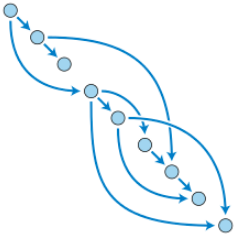
\includegraphics[height=1.5in]{../images/SortedDAG}}

\vfill
An auto-regressive model is locally normalized.

\begin{eqnarray*}
  Q_f(\hat{y}) & = & \prod_i \; Q_f(\hat{y}[i]\;|\; \hat{y}[\mathrm{Parents}(i)]) \\
  \\
  Q_f(\hat{y}[i]\;|\; \hat{y}[\mathrm{Parents}(i)])  & = &  \softmax_{\tilde{y}} f(\tilde{y}|\hat{y}[\mathrm{Parents}(i)])
\end{eqnarray*}

\vfill
There are exponentially many possible values for $\hat{y}$ but each softmax is over a tractable-sized set.

\slidetwo{General Markov Random Fields (MRFs)}{are More Challenging}

We can run a CNN with parameters $\Phi$ on the black and white image $x$ to get a Markov random field (MRF) $f_\Phi(x)$ on possible color images.

\vfill
The MRF $f_\Phi(x)$ will determine the probabilities $Q_\Phi(\hat{y}|x) = Q_{f_\Phi(x)}(\hat{y})$.

\slide{Markov Random Fields (MRFs)}

\centerline{\includegraphics[height = 2in]{../images/colorization}}

\vfill
$\hat{y}[i]$ is the color value of pixel $i$ in image $\hat{y}$.

\vfill
$\hat{y}[(i,j)]$ is the pair $(\hat{y}[i],\hat{y}[j])$ for neighboring pixels $i$ and $j$.

\slide{Markov Random Fields (MRFs)}

\centerline{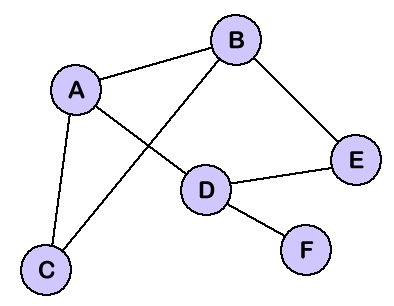
\includegraphics[height= 1.5in]{../images/Graph}}

$$f(\hat{y}) = \sum_{i \in \mathrm{Nodes}}\; f[i,\hat{y}[i]]\; + \sum_{(i,j) \in \mathrm{Edges}}\;f[(i,j),\hat{y}[(i,j)]]$$

\vfill
\centerline{Node Potentials \hspace{4em}Edge Potentials}


\slide{Exponential Softmax}

\begin{eqnarray*}
Q_{f}(\hat{y}) & = & \softmax_{\hat{y}}\;f(\hat{y})
\end{eqnarray*}

\vfill
$$Q_f(\hat{y}) = \frac{1}{Z} \; e^{f(\hat{y})} \;\;\;\;\;\;\;  Z = \sum_{\hat{y}}\;e^{f(\hat{y})}$$

\vfill
$$f(\hat{y}) = \sum_{i \in \mathrm{Nodes}}\; f[i,\hat{y}[i]]\; + \sum_{(i,j) \in \mathrm{Edges}}\;f[(i,j),\hat{y}[(i,j)]]$$

\slide{Hyper-Graphs: More General and More Concise}

A hyper-edge is a subset of nodes.

\vfill
\centerline{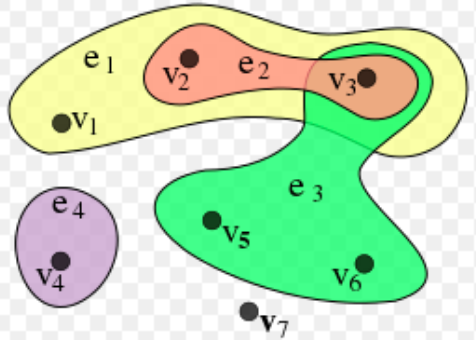
\includegraphics[height = 1.5in]{../images/HyperGraph}}

$$f(\hat{y}) = \sum_{i \in \mathrm{Nodes}}\; f[i,\hat{y}[i]]\; + \sum_{(i,j) \in \mathrm{Edges}}\;f[(i,j),\hat{y}[(i,j)]]$$

\vfill


$${\color{red} f(\hat{y}) = \sum_{\alpha \in \mathrm{HyperEdges}}  \; f[\alpha,\hat{y}[\alpha]]}$$

\slide{Back-Propagation Through An Exponential Softmax}

\begin{eqnarray*}
\Phi^* & =  & \argmin_\Phi \;\;E_{(x,y) \sim \mathrm{Pop}}  -\log Q_\Phi(y|x) \\
\\
 & = &  \argmin_\Phi \;\;E_{(x,y) \sim \mathrm{Pop}}  -\log Q_{f_\Phi(x)}(y)
 \end{eqnarray*}

\vfill
We need to back-propagate through the softmax to get $f.\grad$.

\vfill
$f$ is a tensor containing the numbers $f[\alpha,\tilde{y}]$ where $\tilde{y}$ is a possible value of $\hat{y}[\alpha]$.

\vfill
$$f.\grad[\alpha,\tilde{y}] = \frac{- \partial \log Q_f(y)}{\partial f[\alpha,\tilde{y}]}$$

\slide{Back-Propagation Through An Exponential Softmax}

\bigskip
\begin{eqnarray*}
  \mathrm{loss}(f,y) & = & - \ln \left(\frac{1}{Z(f)}\;e^{f(y)}\right) \\
  \\
  & = & \ln Z(f) - f(y) \\
  \\
  \\
  f.\mathrm{grad}[\alpha,\tilde{y}]
    & = & \left(\frac{1}{Z} \sum_{\hat{y}} e^{f(\hat{y})} \left(\partial f(\hat{y})/\partial f[\alpha,\tilde{y}]\right)\right)
    - \left(\partial f(y) /\partial f[\alpha,\tilde{y}]\right)
\end{eqnarray*}

\slide{Back-Propagation Through An Exponential Softmax}

\bigskip
\begin{eqnarray*}
    f.\mathrm{grad}[\alpha,\tilde{y}]
    & = & \left(\frac{1}{Z} \sum_{\hat{y}} e^{f(\hat{y})} \left(\partial f(\hat{y})/\partial f[\alpha,\tilde{y}]\right)\right)
    - \left(\partial f(y) /\partial f[\alpha,\tilde{y}]\right)    \\
    \\
    & = & \left(\sum_{\hat{y}} Q_f(\hat{y}) \left(\partial f(\hat{y})/\partial f[\alpha,\tilde{y}]\right)\right)
    - \left(\partial f(y) /\partial f[\alpha,\tilde{y}]\right)    \\
    \\
    & = & E_{\hat{y} \sim Q_f}\bbone[\hat{y}[\alpha] = \tilde{y}]
    - \mathbbm{1}[y[\alpha] = \tilde{y}] \\
    \\
    & = & {\color{red} P_{\hat{y} \sim Q_f}(\hat{y}[\alpha] = \tilde{y})}
      - \mathbbm{1}[y[\alpha] = \tilde{y}]
\end{eqnarray*}

\slideplain{Sufficient Statistics}

\begin{eqnarray*}
    f.\mathrm{grad}[\alpha,\tilde{y}]
    & = &  {\color{red} P_{\hat{y} \sim Q_f}(\hat{y}[\alpha] = \tilde{y})} - \bbone[y[\alpha] = \tilde{y}] \\
\end{eqnarray*}

\vfill
To compute $f.\mathrm{grad}$ it suffices to compute ${\color{red} P_{\hat{y} \sim Q_f}(\hat{y}[\alpha] = \tilde{y})}$.

\vfill
By (minor) abuse of terminology we will call the quantities ${\color{red} P_{\hat{y} \sim Q_f}(\hat{y}[\alpha] = \tilde{y})}$ the {\bf sufficient statistics}
for $f$.

\vfill
We now focus on computing the sufficient statistics for a given MRF $f$.

\slide{An Aside: Features and Weights}

The indicators $\mathbbm{1}[\hat{y}[\alpha] = \tilde{y}]$ form a 0-1 feature vector $\Psi(\hat{y})$.

\vfill
The tensor $f[\alpha,\;\tilde{y}]$ forms a weight vector.

\begin{eqnarray*}
f(\hat{y}) & = & \sum_\alpha f[\alpha,\hat{y}[\alpha]] \\
\\
& = & \sum_{\alpha,\tilde{y}}\;f[\alpha,\tilde{y}] \mathbbm{1}[\alpha, \hat{y}[\alpha] = \tilde{y}] \\
\\
& = & f^\top \Psi(\hat{y})
\end{eqnarray*}

\slide{An Aside: Features and Weights}

The sufficient statistics  ${\color{red} P_{\hat{y} \sim Q_f}(\hat{y}[\alpha] = \tilde{y})}$ are just the expected value of the features under the distribution
defined by the MRF.

\slide{Belief Propagation}

\begin{eqnarray*}
  f.\mathrm{grad}[\alpha,\tilde{y}] & = & P_{\hat{y} \sim Q_f}\;(\hat{y}[\alpha] = \tilde{y}) - \mathbbm{1}[y[\alpha] = \tilde{y}]
\end{eqnarray*}

\vfill
\centerline{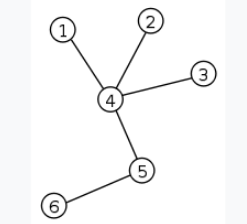
\includegraphics[height= 2in]{../images/Tree}}

\vfill
For trees we can compute $P_{\hat{y} \sim Q_f}\;(\hat{y}[\alpha] = \tilde{y})$ exactly by message passing, aka, belief propagation.

\anaslide{Message Passing}

\centerline{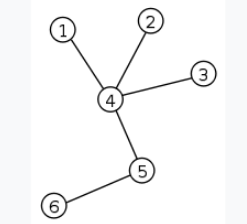
\includegraphics[height=1.5in]{../images/Tree}}

\vfill
For each edge $(i,j)$ there is a message $Z_{i \rightarrow j}$ and a message $Z_{j \rightarrow i}$.

\vfill
Each message is assigns a weight to each node value of the target node.


\vfill
$Z_{j \rightarrow i}[\tilde{y}]$ is the partition function for the subtree attached to $i$ through $j$ and
with $\hat{y}[i]$ restricted to $\tilde{y}$.

\anaslide{Message Passing}

\centerline{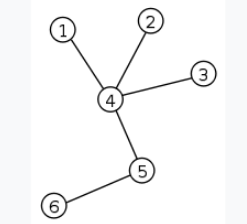
\includegraphics[height=1.5in]{../images/Tree}}

\begin{eqnarray*}
Z(i,\tilde{y}) & \doteq & \sum_{\hat{y}:\; \hat{y}[i] = \tilde{y}} \;e^{f(\hat{y})} \\
\\
& = & e^{f[i,\tilde{y}]} \left(\prod_{j\in N(i)} Z_{j \rightarrow i}[\tilde{y}]\right) \\
\\
{\color{red} P_{\hat{y}\sim Q_f}(\hat{y}[i] = \tilde{y})} & = & Z(i,\tilde{y})/Z,\;\;\;\;\; Z = \sum_{\tilde{y}}\;Z(i,\tilde{y})
\end{eqnarray*}


\slide{Message Passing}

\centerline{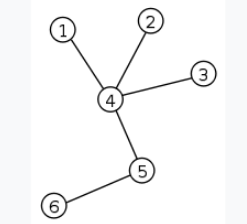
\includegraphics[height=2.0in]{../images/Tree}}

\vfill
\begin{eqnarray*}
  Z_{j\rightarrow i}[\tilde{y}] & = & \sum_{\tilde{y}'}  e^{f[j,\tilde{y}'] + f[\{j,i\},\{\tilde{y}',\tilde{y}\}]}
    \left(\prod_{k \in N(j),\;k \not = i}\;Z_{k\rightarrow j}[\tilde{y}']\right)
\end{eqnarray*}

\anaslide{Message Passing}

\begin{eqnarray*}
Z(\{i,j\},\tilde{y}) & \doteq & \sum_{\hat{y}:\; \hat{y}[\{i,j\}] = \tilde{y}} \;e^{f(\hat{y})} \\
\\
& = & e^{f[i,\tilde{y}[i]] + f[j,\tilde{y}[j]] +f[\{i,j\},\tilde{y}]} \\
& & \prod_{k\in N(i),\;k \not = j} Z_{k \rightarrow i}[\tilde{y}[i]] \\
& & \prod_{k\in N(j),\;k \not = i} Z_{k \rightarrow j}[\tilde{y}[j]] \\
\\
{\color{red} P_{\hat{y}\sim Q_f}(\hat{y}[\{i,j\}] = \tilde{y})} & = & Z(\{i,j\},\tilde{y})/Z
\end{eqnarray*}

\slide{Loopy BP}

Message passing is also called belief propagation (BP).

\vfill
In a graph with cycles it is common to do {\bf Loopy BP}.

\vfill
This is done by initializing all message $Z_{i \rightarrow j}[\tilde{y}] = 1$ and then repeating (until convergence) the updates
\vfill
\begin{eqnarray*}
  Z_{j\rightarrow i}[\tilde{y}] & = & \sum_{\tilde{y}'}  e^{f[j,\tilde{y}'] + f[\{j,i\},\{\tilde{y}',\tilde{y}\}]}
    \left(\prod_{k \in N(j),\;k \not = i}\;Z_{k\rightarrow j}[\tilde{y}']\right)
\end{eqnarray*}

\slide{END}

}
\end{document}

